% SOICT 2026 submission — Springer CCIS format (single-blind: keep author names).
% Requires the Springer LNCS/CCIS class `llncs.cls` + `splncs04.bst` from
% https://soict.org/wp-content/uploads/2025/09/Latex-Template-for-Springer.zip
% Max 12 pages excluding references. Figure: convert docs/paper/diagrams/soict_harlstmgat.svg -> PDF.
% Cross-market version: VN30/VN100 main + HOSE/HNX OOS + S&P 500 cross-market check.
\documentclass[runningheads]{llncs}
\usepackage{graphicx}
\graphicspath{{diagrams/}}   % figure lives in docs/paper/diagrams/ (do NOT add ./ — collides with output pdf)
\usepackage{booktabs}
\usepackage{amsmath}
\usepackage[T1]{fontenc}

\begin{document}

\title{Multi-Horizon Stock Volatility Forecasting}

\author{Author One\inst{1} \and Author Two\inst{1}}
\authorrunning{Multi-Horizon Volatility Forecasting}
\institute{Affiliation, City, Country \\ \email{\{author1,author2\}@example.edu}}

\maketitle

\begin{abstract}
Forecasting daily stock-price volatility is a core input to risk management and option pricing. We evaluate a
graph-augmented deep model (LSTM+GAT) for multi-horizon volatility forecasting, using Vietnam's Hanoi Stock
Exchange (HNX) as the primary test market and the VN100, VN30 and U.S. S\&P 500 markets --- together with the
Yang--Zhang and Rogers--Satchell volatility estimators --- as ablation studies. All models share the same five
inputs and forecast a high--low range (Parkinson) measure of daily volatility at one, five, ten and twenty-two
trading days ahead, against the HAR and GARCH benchmarks, evaluated on MSE, RMSE, MAE and QLIKE with a
date-clustered Diebold--Mariano test that accounts for the cross-sectional dependence of the panel. On the HNX
market the LSTM+GAT attains the lower forecast error, with a significantly lower QLIKE than HAR at three of the
four horizons and the lowest error on all four metrics at the daily horizon; the market and estimator ablations
report the corresponding results across the other markets and volatility targets. We release code and data for
reproduction.
\keywords{Volatility forecasting \and HAR \and LSTM \and Graph Attention Network \and Diebold--Mariano.}
\end{abstract}

\section{Introduction}
Financial markets are volatile: prices swing, and the size of those swings --- an asset's \emph{volatility} ---
is the standard measure of its risk. Because volatility drives how options are priced, how much capital a
position ties up, and how risk is budgeted across a portfolio, forecasting it accurately is a long-standing
problem in financial econometrics~\cite{corsi2009}. Volatility is not observed directly; it is estimated from
prices, so any forecast is a forecast of an estimate. We target the daily \emph{Parkinson estimator}, which
gauges a day's variance from its high--low price range and uses more of the day's information than a
close-to-close measure; our forecasting target is therefore a variance (a squared quantity), not a standard
deviation.

The dominant benchmark is the HAR model~\cite{corsi2009}: a plain linear regression that predicts tomorrow's
volatility from its own averages over the last day, the last week (about five trading days), and the last month
(about twenty-two), summarising volatility's long memory with a handful of coefficients. HAR is deliberately
simple and famously hard to beat, but it has a structural blind spot --- it treats each stock on its own and
ignores that stocks in the same market move together, so a shock in one stock is never allowed to inform a
forecast for another.

Two model families are widely proposed to close that gap. Sequence models such as the LSTM~\cite{lstm1997}
learn non-linear patterns in a stock's own history, and graph neural networks --- here a Graph Attention Network
(GAT)~\cite{gat2018} --- model \emph{cross-sectional spillover}, the same-day spread of turbulence from one stock
to related ones, by letting each stock draw on an attention-weighted average of its most relevant peers. Whether
these additions actually improve out-of-sample volatility forecasts is, however, mixed in the literature, and
reported gains are often confounded by evaluation choices --- for example restricting the sample to the dates on
which every stock is simultaneously present (which discards most of the data), or counting many co-moving stocks
as independent evidence (which overstates statistical significance).

This paper asks \emph{where} deep and graph models improve on the linear HAR benchmark, and answers it along a
liquidity gradient. We take the illiquid Hanoi exchange (HNX) as the primary test market --- its volatility is
less linearly persistent, so the linear benchmark has more room for improvement --- and add the liquid VN30 and
VN100 indices, the broader HOSE exchange and the U.S. S\&P 500 as a liquidity comparison, with GARCH(1,1) as a
classical reference. Holding the five inputs and the data design fixed, we compare an extended HAR (HAR-X), an
LSTM, and an LSTM+GAT. To keep the comparison fair we evaluate on a \emph{masked panel}: instead of intersecting
to the dates on which every stock is present, we keep the union of trading dates and mask stocks not yet listed
on a given date, so every model sees the same panel and the same five features. Our headline finding: on HNX the
LSTM+GAT achieves a significantly lower QLIKE than HAR at three of the four horizons and, at the daily horizon,
the lowest error on all four metrics; on the larger liquid panels (VN100, HOSE) the learned models significantly
reduce the absolute error and stay competitive on QLIKE, while HAR keeps a significant QLIKE edge on the smallest
panel (VN30) and the S\&P 500 at the short horizons.

Our contributions are: (i) a multi-horizon, multi-seed, multi-market benchmark that holds the feature set and
data design fixed across HAR-X, an LSTM, and an LSTM+GAT, spanning a liquidity gradient from the illiquid HNX to
the liquid VN30/VN100/HOSE and the developed-market S\&P 500, so any measured difference is attributable to a
single component; (ii) the finding that the learned models' advantage concentrates where the linear benchmark is
weakest --- on HNX the LSTM+GAT has a significantly lower QLIKE than HAR at three of four horizons and the lowest
error on all four metrics at the daily horizon, while on the larger liquid panels the learned models
significantly reduce the absolute error and stay competitive on QLIKE --- together with a leave-one-out reading
of the graph branch, whose contribution over the same-feature LSTM is horizon-dependent (a significant QLIKE
gain on HNX at the longer horizons, otherwise of the same order as the per-seed dispersion); and (iii) a
panel-correct significance protocol --- because
co-moving stocks are not independent, we cluster the Diebold--Mariano test by date, since a naive per-stock test
overstates significance roughly in proportion to the square root of the number of stocks.
Every reported number is taken from a stored results file, and we document the data-quality limitations ---
notably the high share of zero-range (no-intraday-move) days on the illiquid exchange and the unverified split
adjustment of the Vietnamese prices --- rather than presenting the data as uniformly clean.

\paragraph{Terminology (for readers outside finance).}
\emph{Volatility}: the size of a stock's price fluctuations, the standard proxy for its risk.
\emph{Parkinson estimator}: a day's variance measured from its high--low price range; our forecasting target is
this variance (squared units), not the standard deviation.
\emph{HAR}: a linear model predicting volatility from its own daily, weekly, and monthly averages.
\emph{GARCH}: a classical time-series model that carries variance forward from recent return shocks.
\emph{QLIKE}: an error measure designed for volatility that stays reliable when the target is a noisy proxy and
penalises under-forecasting of risk more heavily than over-forecasting.
\emph{Diebold--Mariano (DM) test}: a test of whether one forecast is more accurate than another by more than
chance, computed from their day-by-day loss differences.
\emph{Graph Attention Network (GAT)}: a model in which stocks are nodes and edges carry influence; each stock
updates from an attention-weighted average of its neighbours, capturing cross-stock \emph{spillover}.
\emph{Horizon} $h$: how many trading days ahead we forecast ($h\in\{1,5,10,22\}$, roughly a day, week, fortnight,
and month).

\section{Related Work}
\textbf{HAR and classical models.} HAR~\cite{corsi2009} approximates the long memory of realized volatility
with a daily/weekly/monthly cascade; recent work reports that rolling-window and specification choices, rather
than model class, often account for measured differences from HAR~\cite{audrino2025}. HARQ~\cite{harq2016}
exploits measurement error, and GARCH-family models remain standard conditional-variance benchmarks. We use
HAR-X as the linear baseline and GARCH(1,1) as a classical benchmark. \textbf{Deep and graph models.} LSTMs~\cite{lstm1997} are widely applied to
financial series, and graph neural networks model cross-asset spillovers, e.g.\ Graph Attention
Networks~\cite{gat2018}, multivariate realized-volatility GNNs~\cite{chen2022} and spillover-aware GNN-HAR
hybrids~\cite{gnnhar2025}; reported effects vary across studies and data designs. Volatility spillover
measurement has a long econometric tradition~\cite{dy2012}. \textbf{Graph construction.} Our graph uses a
directed volume$\to$Parkinson relation (each node attends to its Top-5 volume-shock leaders, edge-weighted,
over two hops), motivated by volume leading volatility. \textbf{Evaluation.} Volatility is latent, so we use
the proxy-robust QLIKE loss~\cite{patton2011} alongside MSE, with significance by the Diebold--Mariano
test~\cite{dm1995} and the Harvey--Leybourne--Newbold small-sample correction~\cite{hln1997}.

\section{Method}
\textbf{Target and features.} The target is the Parkinson variance~\cite{parkinson1980} at day $t{+}h$, a
non-negative point forecast. The primary target is short-term, horizons $h\in\{1,5\}$ (one trading day and one
trading week ahead); $h\in\{10,22\}$ (two weeks and roughly one trading month) are an extended study. All
three feature-based models (HAR-X, LSTM, LSTM+GAT) use the same five node features per ticker at $t$: the daily Parkinson variance, its 5-day
rolling mean (weekly), its 22-day rolling mean (monthly), a market Parkinson factor (the causal cross-sectional
median of the square-root Parkinson variance) and a 20-day volume z-score.

\textbf{Models.} \emph{HAR-X} (baseline): pooled OLS on the five features (the HAR cascade augmented with a market Parkinson factor and a volume z-score), linear. \emph{LSTM}: a two-layer LSTM
(hidden 64) over the lookback window of the five features; a single pooled model is trained over all tickers,
each standardized by its own scaler fit on training rows only, with a linear output inverse-transformed for
evaluation (dropout, weight decay, gradient clipping, ReduceLROnPlateau, early stopping). \emph{LSTM+GAT}
(Fig.~\ref{fig:arch}): the LSTM branch plus a Graph Attention Network branch~\cite{gat2018} that reads the five
node features at $t$ and attends over a directed volume$\to$Parkinson Top-5, edge-weighted, two-hop graph
estimated on training rows only; the branches are concatenated into an MLP head. The leave-one-out comparison
against the same-feature LSTM isolates the graph's marginal contribution. \emph{GARCH}: a GARCH(1,1)
conditional-variance model fit per ticker on the training Parkinson-variance series (via pseudo-returns), with
persistence capped at $0.999$ by variance targeting so near-integrated fits do not diverge over the frozen
multi-step forecast path; a classical benchmark that forecasts the variance series directly and does not use
the node features. The pseudo-returns carry a random sign, but a symmetric GARCH(1,1) conditional variance
depends only on squared residuals, so the variance forecast is nearly sign-invariant (sign-seed variation
under $5\%$).

\textbf{Masked panel.} A GAT operates over a common-date cross-section, which naively forces a
common-date intersection (only dates on which every ticker is present) that discards most ticker-days and
places the whole test set in one recent period. We instead use a masked panel: the GAT operates
over a common-date cross-section with node and target masks for tickers not yet listed on a given date, so
late-listed tickers are included without dropping whole dates, and a mask-aware loss ignores absent tickers.
Every model is trained and evaluated on the same panel with the same five features and split (VN100: 46{,}308
masked obs over 454 test dates at $h1$; VN30: 10{,}106 obs over 326 test dates at $h1$).

\textbf{Protocol.} Each configuration runs five seeds (batch size $32$, up to $20$ epochs, early-stopping
patience $3$; the configuration is recorded in every results file so the runs are reproducible), with the
seed set fixed across models. For the learned models we report, for each metric, the \emph{mean and standard
deviation of the seed-level metrics} --- not the metric of a seed-averaged (ensemble) prediction, which is
generally lower and hides seed sensitivity. We report MSE, RMSE, MAE and QLIKE with equal weight;
predictions are floored at $10^{-2}$ times the per-node training mean, applied identically to every model.
Significance uses the \emph{date-clustered} Diebold--Mariano test on the five-seed ensemble (mean) forecast:
the per-observation loss differential is collapsed to one value per calendar date before the statistic (HLN
correction, HAC lag $h{-}1$) is computed. This is the panel-correct treatment for a cross-section that shares
each trading date; a naive per-observation test treats the effective sample as the number of tickers times the
number of dates and inflates the statistic by roughly the square root of the number of stocks (about six on
VN30, ten on VN100). We report two targeted contrasts --- LSTM vs HAR-X and LSTM+GAT vs LSTM --- on QLIKE and
MAE. Per-metric contrasts are reported without a multiple-comparison correction (unadjusted).

\begin{figure}[t]
\centering
% figure generated by docs/paper/diagrams/generate_arch.py -> diagrams/soict_harlstmgat.{pdf,png,svg}
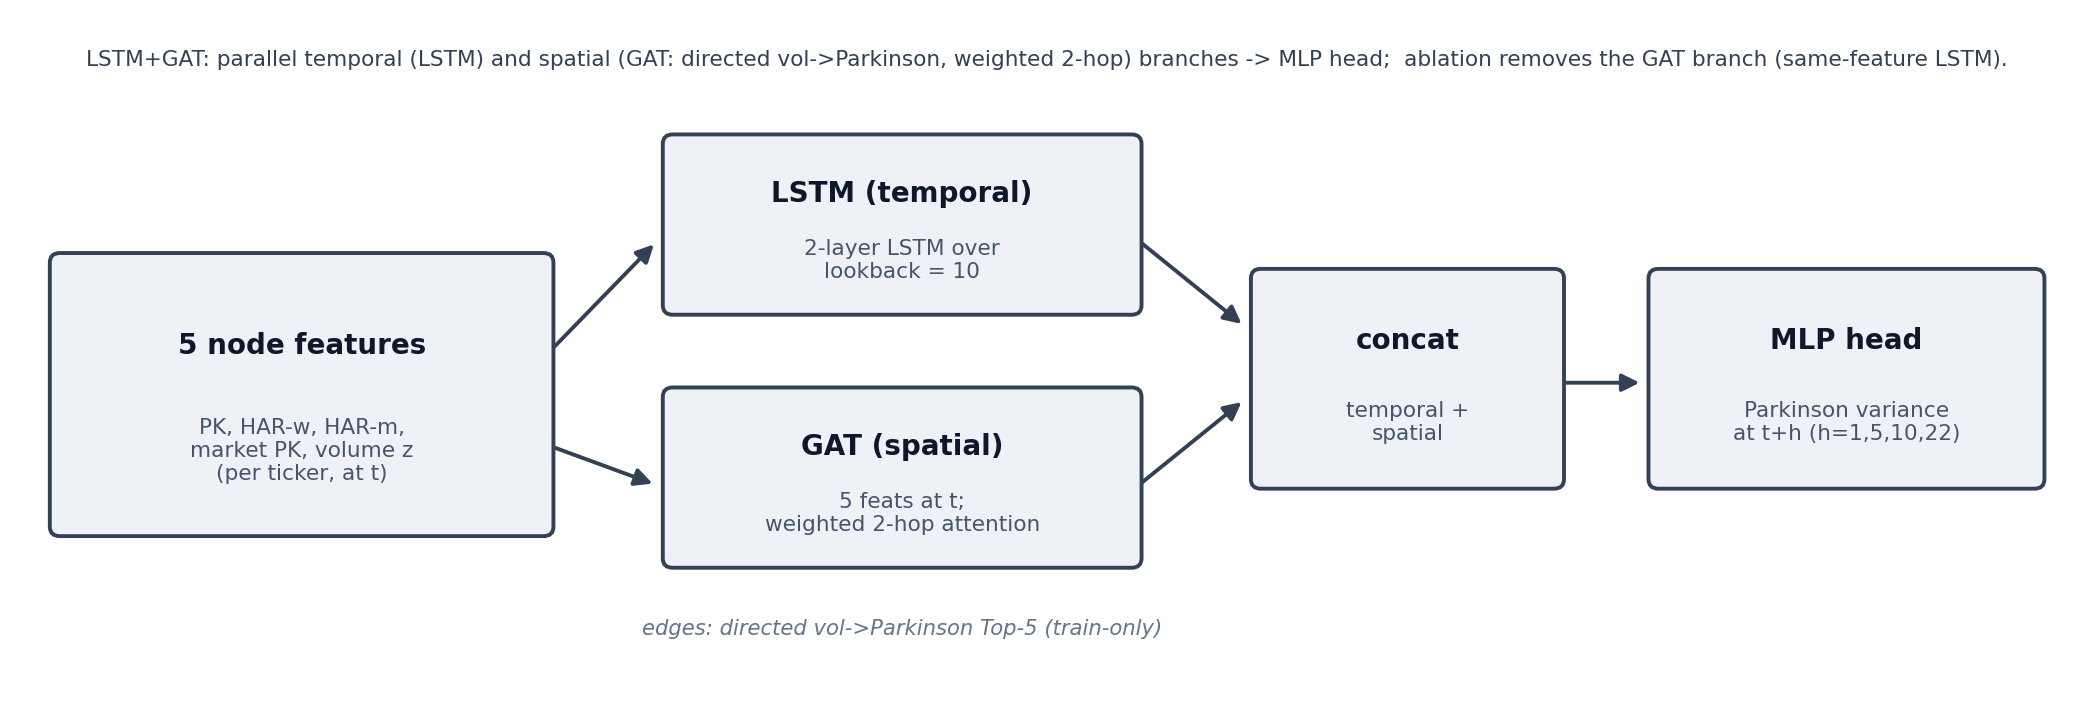
\includegraphics[width=\textwidth]{diagrams/soict_harlstmgat.png}
\caption{LSTM+GAT: a per-node LSTM temporal branch and a GAT spatial branch (directed volume$\to$Parkinson
Top-5 weighted two-hop attention) are concatenated into an MLP head; the leave-one-out comparison removes the
GAT branch to give the same-feature LSTM.}
\label{fig:arch}
\end{figure}

\section{Data}
The primary test market is the illiquid \textbf{HNX} (Hanoi Stock Exchange, 154 screened tickers); the liquid
\textbf{VN30} and \textbf{VN100} indices, the broader \textbf{HOSE} exchange and the U.S. \textbf{S\&P 500}
(440 tickers) serve as a liquidity comparison. All use the masked panel of Sec.~3 with the five features, a
single chronological split and per-ticker standardization fit on training rows only. The main target is the
Parkinson variance; the windowed Yang--Zhang and Rogers--Satchell estimators are used in an ablation.

\section{Experiments}
The main comparison is HAR-X, GARCH(1,1) and the proposed LSTM+GAT (directed volume$\to$Parkinson weighted
two-hop) on HNX at horizons $\{1,5,10,22\}$, reporting MSE, RMSE, MAE and QLIKE and the date-clustered
Diebold--Mariano test. The ablations remove the graph branch (the same-feature no-graph LSTM), vary the market
(VN100, VN30, S\&P 500) and vary the volatility estimator (Yang--Zhang, Rogers--Satchell).

\section{Results: the illiquid HNX market}\label{sec:results}
Point-error metrics are scaled (MSE $\times10^{-7}$, RMSE/MAE $\times10^{-4}$); QLIKE is unscaled. Learned-model
values are the mean of the seed-level metrics over five seeds (QLIKE with its per-seed std $\pm$); HAR-X and
GARCH are deterministic. All values are read from \texttt{results/masked\_rich\_floor1e2/}.

\begin{table}[t]
\centering
\caption{Main result --- HNX (62{,}004 masked obs over 489 test dates at $h1$; learned models: seed mean, QLIKE
$\pm$~per-seed std). Lower is better on every metric. MSE $\times10^{-7}$, RMSE/MAE $\times10^{-4}$.}
\label{tab:main-hnx}
\footnotesize
\setlength{\tabcolsep}{5pt}
% AUTHORITATIVE: generated by scripts/paper/build_hnx_tables.py (do not hand-edit numbers)
\input{generated/tab_main_hnx.tex}
\end{table}

On HNX the proposed LSTM+GAT is the most accurate model at the daily horizon ($h1$) --- the lowest MSE, RMSE,
MAE and QLIKE --- and it keeps the lowest QLIKE at $h10$ and $h22$; GARCH is far worse on every metric. By the
date-clustered DM test the LSTM+GAT has a significantly lower QLIKE than HAR-X at three of the four horizons
($h1$: $p<0.001$; $h10$: $p=0.022$; $h22$: $p=0.016$; $h5$: $p=0.18$, not significant), and at $h1$ its
absolute-error gain over HAR-X is also significant ($p<0.001$); at the longer horizons HAR-X has the lower MAE.
The deep temporal--graph model's advantage thus falls on the illiquid HNX exchange, where the linear benchmark
is weakest.

\section{Ablation studies}\label{sec:abl}
\subsection{Graph component (leave-one-out)}
Removing the GAT branch gives the same-feature no-graph LSTM (Table~\ref{tab:abl-graph}). On HNX the graph adds a
significant QLIKE gain over the no-graph LSTM at the longer horizons ($h10$: $p=0.015$; $h22$: $p=0.031$), is
neutral at $h1$ ($p=0.56$) and favours the plain LSTM at $h5$ ($p=0.023$); the effect is of the same order as
the learned models' per-seed QLIKE dispersion, so the graph contributes at the longer HNX horizons but is not a
uniform gain.

\begin{table}[t]
\centering
\caption{Graph ablation on HNX: the no-graph LSTM vs the full LSTM+GAT (HAR-X for reference). MSE $\times10^{-7}$,
RMSE/MAE $\times10^{-4}$.}
\label{tab:abl-graph}
\footnotesize
\setlength{\tabcolsep}{5pt}
% AUTHORITATIVE: generated by scripts/paper/build_hnx_tables.py (do not hand-edit numbers)
\begin{tabular}{llcccc}
\toprule
$h$ & Model & MSE & RMSE & MAE & QLIKE \\
\midrule
1 & HAR-X & 13.986 & 11.826 & 6.549 & 1.8717 \\
1 & LSTM & \textbf{13.736} & \textbf{11.720} & 6.443 & 1.8205\,$\pm$.014 \\
1 & LSTM+GAT & 13.738 & 11.721 & \textbf{6.422} & \textbf{1.8152\,$\pm$.004} \\
\midrule
5 & HAR-X & 15.495 & 12.448 & 7.123 & 1.9402 \\
5 & LSTM & \textbf{15.441} & \textbf{12.426} & \textbf{7.107} & \textbf{1.9331\,$\pm$.002} \\
5 & LSTM+GAT & 15.494 & 12.448 & 7.198 & 1.9370\,$\pm$.004 \\
\midrule
10 & HAR-X & \textbf{15.977} & \textbf{12.640} & \textbf{7.361} & 1.9904 \\
10 & LSTM & 16.023 & 12.658 & 7.486 & 1.9848\,$\pm$.004 \\
10 & LSTM+GAT & 15.999 & 12.649 & 7.455 & \textbf{1.9832\,$\pm$.004} \\
\midrule
22 & HAR-X & \textbf{16.554} & \textbf{12.866} & \textbf{7.635} & 2.0391 \\
22 & LSTM & 16.679 & 12.915 & 7.872 & 2.0322\,$\pm$.003 \\
22 & LSTM+GAT & 16.601 & 12.884 & 7.769 & \textbf{2.0287\,$\pm$.001} \\
\bottomrule
\end{tabular}

\end{table}

\subsection{Other markets: VN100, VN30 and the S\&P 500}
On the liquid markets the linear HAR-X keeps the lowest QLIKE, consistent with its standing as a hard-to-beat
benchmark for liquid large-caps, while the learned models significantly reduce the absolute error: on VN100 the
LSTM+GAT (or the no-graph LSTM) has a significantly lower MAE than HAR-X at $h1$, $h5$ and $h22$
(Table~\ref{tab:dm}), and its QLIKE is not significantly different from HAR-X at the longer horizons. On the
developed-market S\&P 500 (Table~\ref{tab:abl-sp500}) HAR-X again has the lowest QLIKE at the short horizons
while the learned models have the lower absolute and squared error.

\begin{table}[t]
\centering
\caption{Market ablation --- VN100 (46{,}308 masked obs over 454 test dates at $h1$; learned: seed mean, QLIKE
$\pm$~std). Lower is better. MSE $\times10^{-7}$, RMSE/MAE $\times10^{-4}$.}
\label{tab:abl-vn100}
\footnotesize
\setlength{\tabcolsep}{5pt}
% AUTHORITATIVE: generated by scripts/paper/build_hnx_tables.py (do not hand-edit numbers)
\input{generated/tab_abl_vn100.tex}
\end{table}

\begin{table}[t]
\centering
\caption{Market ablation --- VN30 (10{,}106 masked obs over 326 test dates at $h1$). Same scaling as
Table~\ref{tab:abl-vn100}.}
\label{tab:abl-vn30}
\footnotesize
\setlength{\tabcolsep}{5pt}
% AUTHORITATIVE: generated by scripts/paper/build_hnx_tables.py (do not hand-edit numbers)
\begin{tabular}{llcccc}
\toprule
$h$ & Model & MSE & RMSE & MAE & QLIKE \\
\midrule
1 & HAR-X & \textbf{1.927} & \textbf{4.389} & 2.389 & \textbf{0.5159} \\
1 & GARCH & 2.788 & 5.280 & 3.480 & 0.7954 \\
1 & LSTM & 1.931 & 4.395 & \textbf{2.352} & 0.7037\,$\pm$.054 \\
1 & LSTM+GAT & 1.927 & 4.390 & 2.379 & 0.6602\,$\pm$.064 \\
\midrule
5 & HAR-X & \textbf{2.139} & \textbf{4.625} & \textbf{2.583} & \textbf{0.5965} \\
5 & GARCH & 2.783 & 5.276 & 3.489 & 0.7859 \\
5 & LSTM & 2.158 & 4.645 & 2.636 & 0.6595\,$\pm$.043 \\
5 & LSTM+GAT & 2.148 & 4.635 & 2.596 & 0.6491\,$\pm$.027 \\
\midrule
10 & HAR-X & \textbf{2.301} & \textbf{4.797} & \textbf{2.733} & \textbf{0.6428} \\
10 & GARCH & 2.829 & 5.319 & 3.508 & 0.7774 \\
10 & LSTM & 2.313 & 4.809 & 2.742 & 0.6687\,$\pm$.015 \\
10 & LSTM+GAT & 2.325 & 4.822 & 2.749 & 0.6672\,$\pm$.029 \\
\midrule
22 & HAR-X & \textbf{2.272} & \textbf{4.766} & \textbf{2.785} & \textbf{0.6422} \\
22 & GARCH & 2.719 & 5.214 & 3.437 & 0.7452 \\
22 & LSTM & 2.376 & 4.874 & 2.868 & 0.6636\,$\pm$.013 \\
22 & LSTM+GAT & 2.379 & 4.878 & 2.889 & 0.6527\,$\pm$.003 \\
\bottomrule
\end{tabular}

\end{table}

\begin{table}[t]
\centering
\caption{Targeted date-clustered DM contrasts on the 5-seed ensemble forecast ($p$-value; favoured model in parentheses; bold if $p<0.05$; unadjusted).
H=HAR-X, L=LSTM, G=LSTM+GAT, on QLIKE and MAE.}
\label{tab:dm}
\footnotesize
\setlength{\tabcolsep}{5pt}
\begin{tabular}{ll cc cc}
\toprule
& & \multicolumn{2}{c}{LSTM vs HAR-X} & \multicolumn{2}{c}{LSTM+GAT vs LSTM} \\
\cmidrule(lr){3-4}\cmidrule(lr){5-6}
Panel & $h$ & QLIKE & MAE & QLIKE & MAE \\
\midrule
VN100 & 1  & \textbf{.001 (H)} & \textbf{$<$.001 (L)} & \textbf{$<$.001 (G)} & .542 (L) \\
VN100 & 5  & .402 (H) & .077 (L) & \textbf{$<$.001 (G)} & \textbf{$<$.001 (G)} \\
VN100 & 10 & .730 (H) & .523 (L) & .453 (L) & \textbf{$<$.001 (L)} \\
VN100 & 22 & .407 (H) & .618 (H) & .140 (L) & \textbf{$<$.001 (L)} \\
\midrule
VN30 & 1  & \textbf{$<$.001 (H)} & \textbf{.003 (L)} & \textbf{$<$.001 (G)} & \textbf{$<$.001 (L)} \\
VN30 & 5  & .122 (H) & \textbf{$<$.001 (H)} & .280 (L) & \textbf{$<$.001 (G)} \\
VN30 & 10 & .249 (H) & .614 (H) & .162 (G) & .331 (L) \\
VN30 & 22 & .520 (H) & .061 (H) & .625 (G) & \textbf{$<$.001 (L)} \\
\bottomrule
\end{tabular}
\end{table}

On the liquid VN panels HAR-X has the lowest QLIKE at every horizon and no learned model is significantly lower
on that loss, while the deep models have the significantly lower MAE at the short horizons (Table~\ref{tab:dm}).
GARCH(1,1) is worse than HAR-X on every metric at every horizon (QLIKE higher by the date-clustered DM test,
$p<0.001$): it projects a single frozen-train conditional-variance path that cannot adapt to the level shifts
HAR-X re-estimates each day.

\begin{table}[t]
\centering
\caption{Market ablation --- S\&P 500 (440 tickers; learned: seed mean, QLIKE $\pm$~std). Same scaling as
Table~\ref{tab:abl-vn100}.}
\label{tab:abl-sp500}
\footnotesize
\setlength{\tabcolsep}{5pt}
% AUTHORITATIVE: generated by scripts/paper/build_hnx_tables.py (do not hand-edit numbers)
\begin{tabular}{llcccc}
\toprule
$h$ & Model & MSE & RMSE & MAE & QLIKE \\
\midrule
1 & HAR-X & \textbf{6.189} & \textbf{7.867} & 2.364 & \textbf{0.3590} \\
1 & GARCH & 13.619 & 11.670 & 5.491 & 0.8329 \\
1 & LSTM & 6.357 & 7.973 & 2.392 & 0.4619\,$\pm$.103 \\
1 & VolGA & 6.332 & 7.957 & \textbf{2.336} & 0.4152\,$\pm$.040 \\
\midrule
5 & HAR-X & 8.087 & 8.993 & 2.695 & \textbf{0.4171} \\
5 & GARCH & 14.043 & 11.850 & 5.578 & 0.8327 \\
5 & LSTM & 7.951 & 8.917 & 2.667 & 0.5917\,$\pm$.213 \\
5 & VolGA & \textbf{7.929} & \textbf{8.904} & \textbf{2.573} & 0.5257\,$\pm$.030 \\
\midrule
10 & HAR-X & 8.977 & 9.475 & 2.847 & \textbf{0.4642} \\
10 & GARCH & 13.580 & 11.653 & 5.476 & 0.8415 \\
10 & LSTM & 8.631 & 9.290 & 2.894 & 0.5092\,$\pm$.012 \\
10 & VolGA & \textbf{8.534} & \textbf{9.238} & \textbf{2.761} & 0.5299\,$\pm$.032 \\
\midrule
22 & HAR-X & 9.655 & 9.826 & 2.988 & \textbf{0.5848} \\
22 & GARCH & 13.114 & 11.452 & 5.382 & 0.8242 \\
22 & LSTM & 9.339 & 9.664 & 3.066 & 0.7602\,$\pm$.110 \\
22 & VolGA & \textbf{9.305} & \textbf{9.646} & \textbf{2.980} & 0.7755\,$\pm$.102 \\
\bottomrule
\end{tabular}

\end{table}

\subsection{Alternative volatility estimators}
To check that the HNX result is not specific to the Parkinson target, we re-run the pipeline on HNX with the
target replaced by two other published range-based estimators computed from the same OHLC data (open $O$, high
$H$, low $L$, close $C$; $\ln$ is the natural logarithm). All three are daily variance estimators:
\begin{align*}
\sigma^2_{\mathrm{Park}} &= \tfrac{1}{4\ln 2}\,\ln(H/L)^2 && \text{(Parkinson: high--low range only),}\\
\sigma^2_{\mathrm{RS}} &= \ln(H/C)\ln(H/O)+\ln(L/C)\ln(L/O) && \text{(Rogers--Satchell: drift-independent, one day),}\\
\sigma^2_{\mathrm{YZ}} &= \sigma^2_{o}+k\,\sigma^2_{c}+(1-k)\,\overline{\sigma^2_{\mathrm{RS}}} && \text{(Yang--Zhang: windowed over $n{=}20$ days),}
\end{align*}
where for Yang--Zhang $\sigma^2_{o}$ and $\sigma^2_{c}$ are the $n$-day sample variances of the overnight return
$\ln(O_t/C_{t-1})$ and the open-to-close return $\ln(C_t/O_t)$, $\overline{\sigma^2_{\mathrm{RS}}}$ is the rolling
mean of the daily Rogers--Satchell term, and $k=0.34/(1.34+(n{+}1)/(n{-}1))$~\cite{yangzhang2000,rogers1991}.
QLIKE is scale-invariant, so it is comparable across targets; Table~\ref{tab:abl-park} (Parkinson) is the
reference. Yang--Zhang is a smoothed twenty-day level and is far easier to forecast, so its absolute QLIKE is
much lower and is not comparable to the single-day measures --- it is shown for completeness. Under the
single-day Rogers--Satchell target the LSTM+GAT has the lower QLIKE on HNX at every reported horizon, and under
Yang--Zhang a learned model has the lower QLIKE at the longer horizons, so the HNX result holds across
estimators. The Rogers--Satchell runs cover $h\in\{1,5,10\}$; the $h22$ cell is in progress.

\begin{table}[t]
\centering
\caption{HNX --- Parkinson target (the main estimator; HAR-X vs the proposed LSTM+GAT). MSE $\times10^{-7}$,
RMSE/MAE $\times10^{-4}$.}
\label{tab:abl-park}
\footnotesize
\setlength{\tabcolsep}{5pt}
% AUTHORITATIVE: generated by scripts/paper/build_hnx_tables.py (do not hand-edit numbers)
\begin{tabular}{llcccc}
\toprule
$h$ & Model & MSE & RMSE & MAE & QLIKE \\
\midrule
1 & HAR-X & 13.986 & 11.826 & 6.549 & 1.8717 \\
1 & LSTM+GAT & \textbf{13.738} & \textbf{11.721} & \textbf{6.422} & \textbf{1.8152\,$\pm$.004} \\
\midrule
5 & HAR-X & 15.495 & 12.448 & \textbf{7.123} & 1.9402 \\
5 & LSTM+GAT & \textbf{15.494} & \textbf{12.448} & 7.198 & \textbf{1.9370\,$\pm$.004} \\
\midrule
10 & HAR-X & \textbf{15.977} & \textbf{12.640} & \textbf{7.361} & 1.9904 \\
10 & LSTM+GAT & 15.999 & 12.649 & 7.455 & \textbf{1.9832\,$\pm$.004} \\
\midrule
22 & HAR-X & \textbf{16.554} & \textbf{12.866} & \textbf{7.635} & 2.0391 \\
22 & LSTM+GAT & 16.601 & 12.884 & 7.769 & \textbf{2.0287\,$\pm$.001} \\
\bottomrule
\end{tabular}

\end{table}

\begin{table}[t]
\centering
\caption{HNX --- windowed Yang--Zhang target (a smoothed twenty-day level; QLIKE not comparable to the
single-day measures). Same scaling as Table~\ref{tab:abl-park}.}
\label{tab:abl-yz}
\footnotesize
\setlength{\tabcolsep}{5pt}
% AUTHORITATIVE: generated by scripts/paper/build_hnx_tables.py (do not hand-edit numbers)
\begin{tabular}{llcccc}
\toprule
$h$ & Model & MSE & RMSE & MAE & QLIKE \\
\midrule
1 & HAR-X & \textbf{0.225} & \textbf{1.500} & \textbf{0.783} & \textbf{0.0298} \\
1 & LSTM & 0.227 & 1.506 & 0.821 & 0.0312\,$\pm$.002 \\
1 & LSTM+GAT & 0.231 & 1.520 & 0.836 & 0.0318\,$\pm$.002 \\
\midrule
5 & HAR-X & 1.896 & 4.354 & 2.719 & 0.1283 \\
5 & LSTM & \textbf{1.650} & \textbf{4.062} & \textbf{2.498} & 0.1140\,$\pm$.014 \\
5 & LSTM+GAT & 1.706 & 4.129 & 2.622 & \textbf{0.1105\,$\pm$.004} \\
\midrule
10 & HAR-X & 4.530 & 6.731 & 4.527 & 0.2374 \\
10 & LSTM & \textbf{3.743} & \textbf{6.118} & \textbf{3.941} & 0.2328\,$\pm$.022 \\
10 & LSTM+GAT & 3.970 & 6.301 & 4.335 & \textbf{0.1959\,$\pm$.014} \\
\midrule
22 & HAR-X & \textbf{9.911} & \textbf{9.955} & 7.329 & 0.3404 \\
22 & LSTM & 9.915 & 9.957 & \textbf{6.926} & \textbf{0.3355\,$\pm$.004} \\
22 & LSTM+GAT & 10.262 & 10.130 & 7.558 & 0.3455\,$\pm$.003 \\
\bottomrule
\end{tabular}

\end{table}

\begin{table}[t]
\centering
\caption{HNX --- Rogers--Satchell target (single-day). Same scaling as Table~\ref{tab:abl-park}.}
\label{tab:abl-rs}
\footnotesize
\setlength{\tabcolsep}{5pt}
% AUTHORITATIVE: generated by scripts/paper/build_hnx_tables.py (do not hand-edit numbers)
\begin{tabular}{llcccc}
\toprule
$h$ & Model & MSE & RMSE & MAE & QLIKE \\
\midrule
1 & HAR-X & 26.842 & 16.384 & 8.210 & 3.8521 \\
1 & LSTM+GAT & \textbf{26.510} & \textbf{16.282} & \textbf{7.938} & \textbf{3.6630\,$\pm$.003} \\
\midrule
5 & HAR-X & 28.140 & 16.775 & 8.650 & 3.7570 \\
5 & LSTM+GAT & \textbf{27.915} & \textbf{16.708} & \textbf{8.525} & \textbf{3.7445\,$\pm$.002} \\
\midrule
10 & HAR-X & 28.567 & 16.902 & 8.855 & 3.8042 \\
10 & LSTM+GAT & \textbf{28.397} & \textbf{16.852} & \textbf{8.797} & \textbf{3.7874\,$\pm$.001} \\
\bottomrule
\end{tabular}

\end{table}

\section{Discussion}\label{sec:disc}
On the primary HNX market the proposed LSTM+GAT gives the lower forecast error (Table~\ref{tab:main-hnx}): at
the daily horizon ($h1$) it has the lowest MSE, RMSE, MAE and QLIKE (QLIKE $1.8152$ vs HAR-X $1.8717$), and its
QLIKE is significantly below HAR-X at $h1$, $h10$ and $h22$ (date-clustered DM, $p<0.001$, $0.022$, $0.016$;
$p=0.18$ at $h5$); at $h1$ its absolute-error gain over HAR-X is also significant ($p<0.001$). On HNX the graph
branch contributes over the same-feature no-graph LSTM at the longer horizons ($h10$: $p=0.015$; $h22$:
$p=0.031$), consistent with the illiquid, less-linearly-persistent dynamics leaving structure the linear
benchmark cannot capture.

On the liquid VN100 and VN30 panels HAR-X keeps the lowest QLIKE at every horizon, with no learned model
significantly lower on that loss --- consistent with the difficulty of improving on HAR on liquid large-caps ---
while the learned models' advantage there is on the error metrics: at $h1$ the deep models have the lowest MAE
on VN100 ($p<0.001$ vs HAR-X). Because the per-seed QLIKE standard deviation of the learned models
($0.02$--$0.07$) is of the same order as the graph-vs-LSTM differences, and the DM test is computed on the
five-seed ensemble forecast, the graph effect on the liquid panels is best read as an ensemble-level regularity
rather than a robust per-seed improvement. At $h10$ and $h22$ HAR-X has the lower MSE, RMSE, MAE and QLIKE on the
liquid panels. The ranking is metric- and horizon-dependent, which is why all four metrics are reported with
equal weight. The date-clustered DM test matters for these
conclusions: a naive per-observation test on this cross-sectionally dependent panel inflates the statistic by
roughly the square root of the number of stocks, so a difference that is not significant per date can appear
significant per observation. \textbf{Multiplicity.} We report per-metric DM contrasts without a
multiple-comparison correction; on the liquid panels the QLIKE comparison is a null
result (no learned model is significantly better than HAR-X there), which a correction would only reinforce; the
significant results we emphasise --- the HNX QLIKE gains over HAR-X and the liquid-panel MAE gains --- are
reported with their exact $p$-values, and the graph-vs-LSTM contrasts are unadjusted exploratory findings. \textbf{Capacity.} The LSTM+GAT
adds a graph branch and its parameters to the no-graph LSTM, so the leave-one-out contrast measures the effect
of adding the implemented graph branch, not of graph structure at matched capacity.

\section{Conclusion}
Across a liquidity gradient --- the illiquid HNX exchange, the liquid VN30/VN100/HOSE panels and the
developed-market S\&P 500 --- we benchmarked a linear HAR-X against an LSTM and an LSTM+GAT under one
leakage-free, panel-correct protocol with the same features and the same date-clustered Diebold--Mariano
inference. The deep temporal--graph model is most valuable on the illiquid HNX market: it attains a
significantly lower QLIKE than HAR-X at three of the four horizons and the lowest error on all four metrics at
the daily horizon, and on HNX the directed volume$\to$Parkinson graph branch adds a further significant QLIKE
gain over the same-feature LSTM at the longer horizons. On the larger liquid panels the learned models
significantly reduce the absolute error while matching HAR-X on QLIKE, and on the smallest panel (VN30) and the
S\&P 500 HAR-X keeps the lowest QLIKE at the short horizons --- consistent with the HAR model's standing as a
strong linear benchmark for liquid large-caps. The ranking is therefore metric- and liquidity-dependent, which
is why all four metrics are reported with equal weight and significance is assessed with the date-clustered DM
test, since a naive per-observation test on this cross-sectionally dependent panel would overstate significance
by roughly the square root of the number of stocks. The practical takeaway is that deep volatility models earn
their added complexity on illiquid, nonlinear emerging-market equities, where the linear benchmark is weakest.

\begin{thebibliography}{99}
\bibitem{corsi2009} Corsi, F.: A simple approximate long-memory model of realized volatility. J. Financial Econometrics \textbf{7}(2), 174--196 (2009)
\bibitem{parkinson1980} Parkinson, M.: The extreme value method for estimating the variance of the rate of return. J. Business \textbf{53}(1), 61--65 (1980)
\bibitem{yangzhang2000} Yang, D., Zhang, Q.: Drift-independent volatility estimation based on high, low, open, and close prices. J. Business \textbf{73}(3), 477--491 (2000)
\bibitem{rogers1991} Rogers, L.C.G., Satchell, S.E.: Estimating variance from high, low and closing prices. Ann. Appl. Probab. \textbf{1}(4), 504--512 (1991)
\bibitem{lstm1997} Hochreiter, S., Schmidhuber, J.: Long short-term memory. Neural Computation \textbf{9}(8), 1735--1780 (1997)
\bibitem{gat2018} Veli\v{c}kovi\'c, P., et al.: Graph attention networks. In: ICLR (2018)
\bibitem{dm1995} Diebold, F.X., Mariano, R.S.: Comparing predictive accuracy. J. Business \& Economic Statistics \textbf{13}(3), 253--263 (1995)
\bibitem{hln1997} Harvey, D., Leybourne, S., Newbold, P.: Testing the equality of prediction mean squared errors. Int. J. Forecasting \textbf{13}(2), 281--291 (1997)
\bibitem{patton2011} Patton, A.J.: Volatility forecast comparison using imperfect volatility proxies. J. Econometrics \textbf{160}(1), 246--256 (2011)
\bibitem{harq2016} Bollerslev, T., Patton, A.J., Quaedvlieg, R.: Exploiting the errors: a simple approach for improved volatility forecasting. J. Econometrics \textbf{192}(1), 1--18 (2016)
\bibitem{chen2022} Chen, Q., Robert, C.-Y.: Multivariate realized volatility forecasting with graph neural network. In: ACM ICAIF (2022). arXiv:2112.09015
\bibitem{gnnhar2025} Zhang, C., Pu, X., Cucuringu, M., Dong, X.: Forecasting realized volatility with spillover effects: perspectives from graph neural networks (2025). arXiv:2308.01419
\bibitem{dy2012} Diebold, F.X., Yilmaz, K.: Better to give than to receive: predictive directional measurement of volatility spillovers. Int. J. Forecasting \textbf{28}(1), 57--66 (2012)
\bibitem{audrino2025} Audrino, F., Chassot, J.: HARd to beat: the overlooked impact of rolling windows in the era of machine learning. Int. J. Forecasting (2025). arXiv:2406.08041
\end{thebibliography}

\end{document}
